\chapter{Objektorientierte Analyse und Design}

Im Folgenden wird die objektorientierte Analyse, kurz OOA, beschrieben. In der Analyse geht es darum, die Anforderungen an die Anwendung unter anderem grafisch in Diagrammen zu erfassen und zu beschreiben, mit dem Ziel, ein objektorientiertes Analyse-Modell als Ergebnis zu erhalten. Anschließend wird im objektorientierten Design, kurz OOD, das in der Analyse erstellte Modell weiterentwickelt und in eine konkrete Softwarearchitektur überführt, die dann als direkte Implementierungsvorlage dient\footcite{SWTBalzert}.
\\
\\
Zunächst werden in der objektorientierten Analyse das statische Modell und das dynamische Modell beschrieben. In der Regel wird das statische Modell anhand eines Klassendiagramms beschrieben, in dem alle notwendigen Klassen und Beziehungen dargestellt werden, um die in der Anforderungsanalyse definierten Anforderungen an die Anwendung umzusetzen. Die dynamischen Modelle beschreiben hingegen Abläufe bei der Nutzung der Anwendung. 

\section{Dynamisches Modell (OOA)}

Die Interaktionen des Benutzers mit der Funktionstest-Anwendung werden in folgendem Use-Case-Diagramm (Abbildung \ref{fig:Use_Case}) dargestellt. Links ist der allgemeine Benutzer dargestellt. Der Benutzer der Funktionstest-Anwendung muss eine Auflistung der Sensoren angezeigt bekommen, die er testen kann. Er muss die Kamera des Smartphones benutzen können, das heißt, dass er Fotos schießen und diese auch speichern können soll. Entscheidet sich der Benutzer dazu Sensoren zu testen, so kann er folgende Aktivitäten durchführen: Der Benutzer kann durch Bewegungen seines Smartphones den Beschleunigungssensor und mit diesem zusammen den Lagesensor und das Gyroskop testen. Er kann sich auf einer Karte seinen aktuellen Standort anzeigen lassen. Mit Hilfe des im Smartphone integrierten Magnetometers soll sich der Benutzer den magnetischen Nordpol anzeigen lassen können. Als letzten Sensor soll der Benutzer auch den Näherungssensor testen können. Die Fotos, die der Benutzer mit der Kamerafunktion aufgenommen hat, soll er sich auch später ansehen und auch wieder löschen können. Als letztes gibt es noch eine Funktion, mit der sich der Benutzer das Logging der Anwendung in einem Textdokument anzeigen zu lassen kann und eine Funktion, die es dem Benutzer ermöglicht das Farbschema des Designs der Anwendung zu ändern.  

\begin{figure}[h]
	\centering
	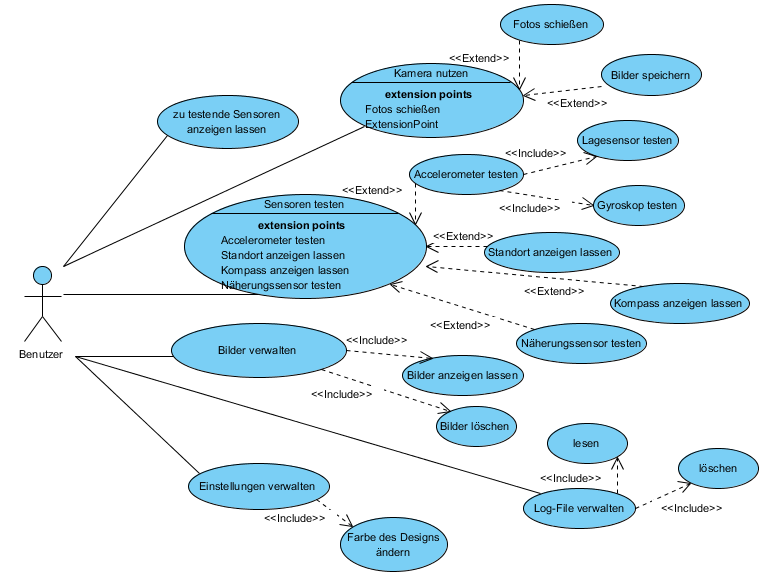
\includegraphics[width=1\textwidth]{Bilder/Use_Case.PNG}
	\caption{Funktionstest-Anwendung: Use-Case Diagramm}
	\label{fig:Use_Case}
\end{figure}

\section{Statisches Modell (OOA)}

Die Funktionstest-Anwendung wird einmal nativ und anschließend mit 5 unterschiedlichen Frameworks entwickelt, was bedeutet, dass sie mit unterschiedlichen Programmiersprachen implementiert werden muss (siehe Kapitel (X)). Dabei sind nicht alle dieser Programmiersprachen objektorientiert und die vorgegebene Architektur der einzelnen Frameworks ist zu diesem Zeitpunkt noch unbekannt. Aus diesem Grund empfiehlt sich an dieser Stelle kein UML Klassendiagramm. Anstelle dessen werden in einem Diagramm die einzelnen Funktionen und die Navigation zu diesen dargestellt (siehe Abbildung \ref{fig:Diagram_1}. So können Hierarchien und Tiefe der Anwendung auch ohne Klassendiagramm analysiert und gezeigt werden.  

\begin{figure}[h]
	\centering
	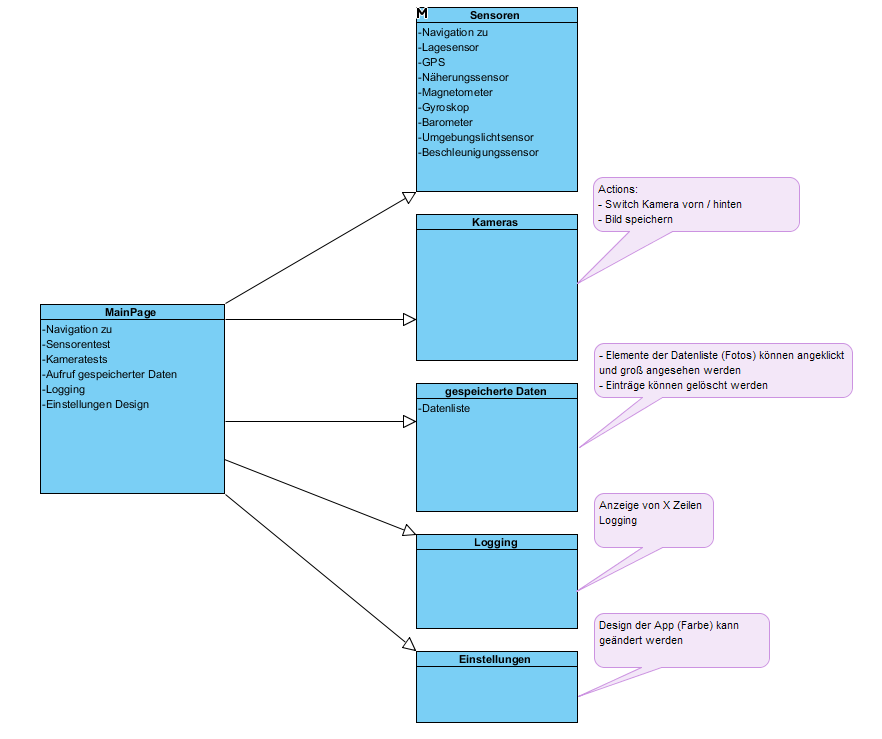
\includegraphics[width=1\textwidth]{Bilder/Diagram_1.PNG}
	\caption{Funktionstest-Anwendung: Navigation Hauptmenü und Beschreibung der einzelnen Funktionen}
	\label{fig:Diagram_1}
\end{figure}

Wie in Abbildung \ref{fig:Diagram_1} zu sehen ist, soll die Anwendung von der 'MainPage' aus starten. Die 'MainPage' ist ein Navigationsmenü, von dem aus der Benutzer zu folgenden Seiten navigieren kann: Zur Sensorliste, zur Kamerafunktion, zu der Seite, welche die vom Benutzer gespeicherten Daten verwaltet, zum Logging-Output und zu einer Einstellungsseite. Die Seite mit der Sensorliste stellt dabei selbst wieder ein Navigationsmenü dar. Navigiert der Benutzer vom Hauptmenü zur Kamerafunktion, so soll er da die Möglichkeit haben, zwischen der Front- und der Rückkamera des Gerätes auszuwählen und Fotos zu schießen. Geschossene Fotos können gespeichert werden. Ein weiterer Menüpunkt des Hauptmenüs führt den Benutzer zur Verwaltung seiner gespeicherten Fotos. Dort soll er durch klicken auf ein Foto dieses vergrößert angezeigt bekommen. Zudem hat er dort die Möglichkeit ausgewählte Bilder wieder zu löschen. Im Menüpunkt 'Logging' wird dem Benutzer das von der Anwendung generierte Logfile angezeigt und im Menüpunkt 'Einstellungen' kann der Benutzer zwischen vorkonfigurierten Farbdesigns für die Anwendung auswählen. 
\\
\\
Im Navigationsmenü der Sensoren kann der Benutzer zu weiteren Funktionen der Anwendung navigieren, wie in Abbildung \ref{fig:Diagram_2} zu sehen ist: 


\begin{figure}[h]
	\centering
	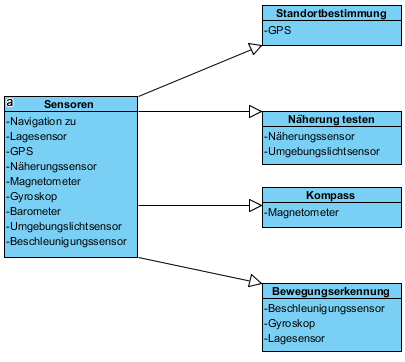
\includegraphics[width=0.6\textwidth]{Bilder/Diagram_2.PNG}
	\caption{Funktionstest-Anwendung: Navigation Sensortests und Beschreibung der einzelnen Funktionen}
	\label{fig:Diagram_2}
\end{figure}
\clearpage
Die 4 Funktionstestseiten, zu denen der Benutzer navigieren kann sind einmal die Standortbestimmung, der Näherungstest, die Kompassanzeige und die Bewegungserkennung (siehe Abbildung \ref{fig:Diagram_2}). Bei der Standortbestimmung wird der GPS-Sensor des Smartphones angesprochen und getestet. Auf dem Display soll eine Weltkarte angezeigt werden mit einem Marker an der Stelle an der der Benutzer sich mit seinem Smartphone befindet. Es soll in die Karte hineingezoomt werden können, damit Ermittlung des Standorts durch das GPS besser überprüft werden kann. Für den Näherungstest werden der Näherungssensor und der Umgebungslichtsensor angesprochen. Hier soll auf dem Display des Smartphones Feedback gegeben werden, sobald sich ein Gegenstand nähert. Das Magnetometer wird bei der Kompassanzeige getestet. Hier bekommt der Benutzer eine Kompassnadel zu Gesicht, welche zum magnetischen Nordpol zeigt. Unter dem Menüpunkt 'Bewegungserkennung' werden der Beschleunigungssensor, das Gyroskop und gegebenenfalls der Lagesensor getestet, sollte es einen separaten geben. 

\section{Datenhaltung (OOD)}

Entsprechend der in Kapitel (X) definierten Anforderungen und der in Kapitel (X) ausgearbeiteten Funktionen der Funktionstest-Anwendung sollen die Fotos, die der Benutzer mit der Kamerafunktion schießt auf dem Smartphone gespeichert werden. Sie sollen im 'External Storage' abgelegt werden. So soll es auch möglich sein aus anderen Anwendungen heraus auf diese Bilder zuzugreifen und sie auf andere Medien zu übertragen. Als Speicherformat für die Fotos wird 'JPG' verwendet. Für die Fotos soll die Anwendung vorher einen eigenen Ordner mit dem Namen 'Feature\_Test\_App' anlegen.

\section{Die grafische Benutzeroberfläche}

Bei der Erstellung des Prototyps für die grafische Benutzeroberfläche wurde darauf geachtet möglichst einige der Standardelemente des 'Material Designs' zu verwenden, welche auch für die native Entwicklung im Android Studio zur Verfügung gestellt werden.
\\
\\
Die Startseite der Anwendung ist das Hauptmenü (Siehe Kapitel(X)). Hier wird der in Kapitel (X) erwähnte 'Navigation Drawer' für die Navigation zu den weiteren Seiten verwendet. Abbildung \ref{fig:Main_Menu} zeigt das Hauptmenü mit geöffneten 'Navigation Drawer', in dem die Navigationsmöglichkeiten zur Kamerafunktion, zu den Sensortests, zur Galerie, dem Logging und den Einstellungen angezeigt werden. Der 'Navigation Drawer' lässt sich einerseits durch Wischen und andererseits über die 'App Bar' öffnen und schließen. Die Sensorauswahl wird ebenfalls mit einem 'Navigation Drawer' realisiert.

\begin{figure}[h]
	\centering
	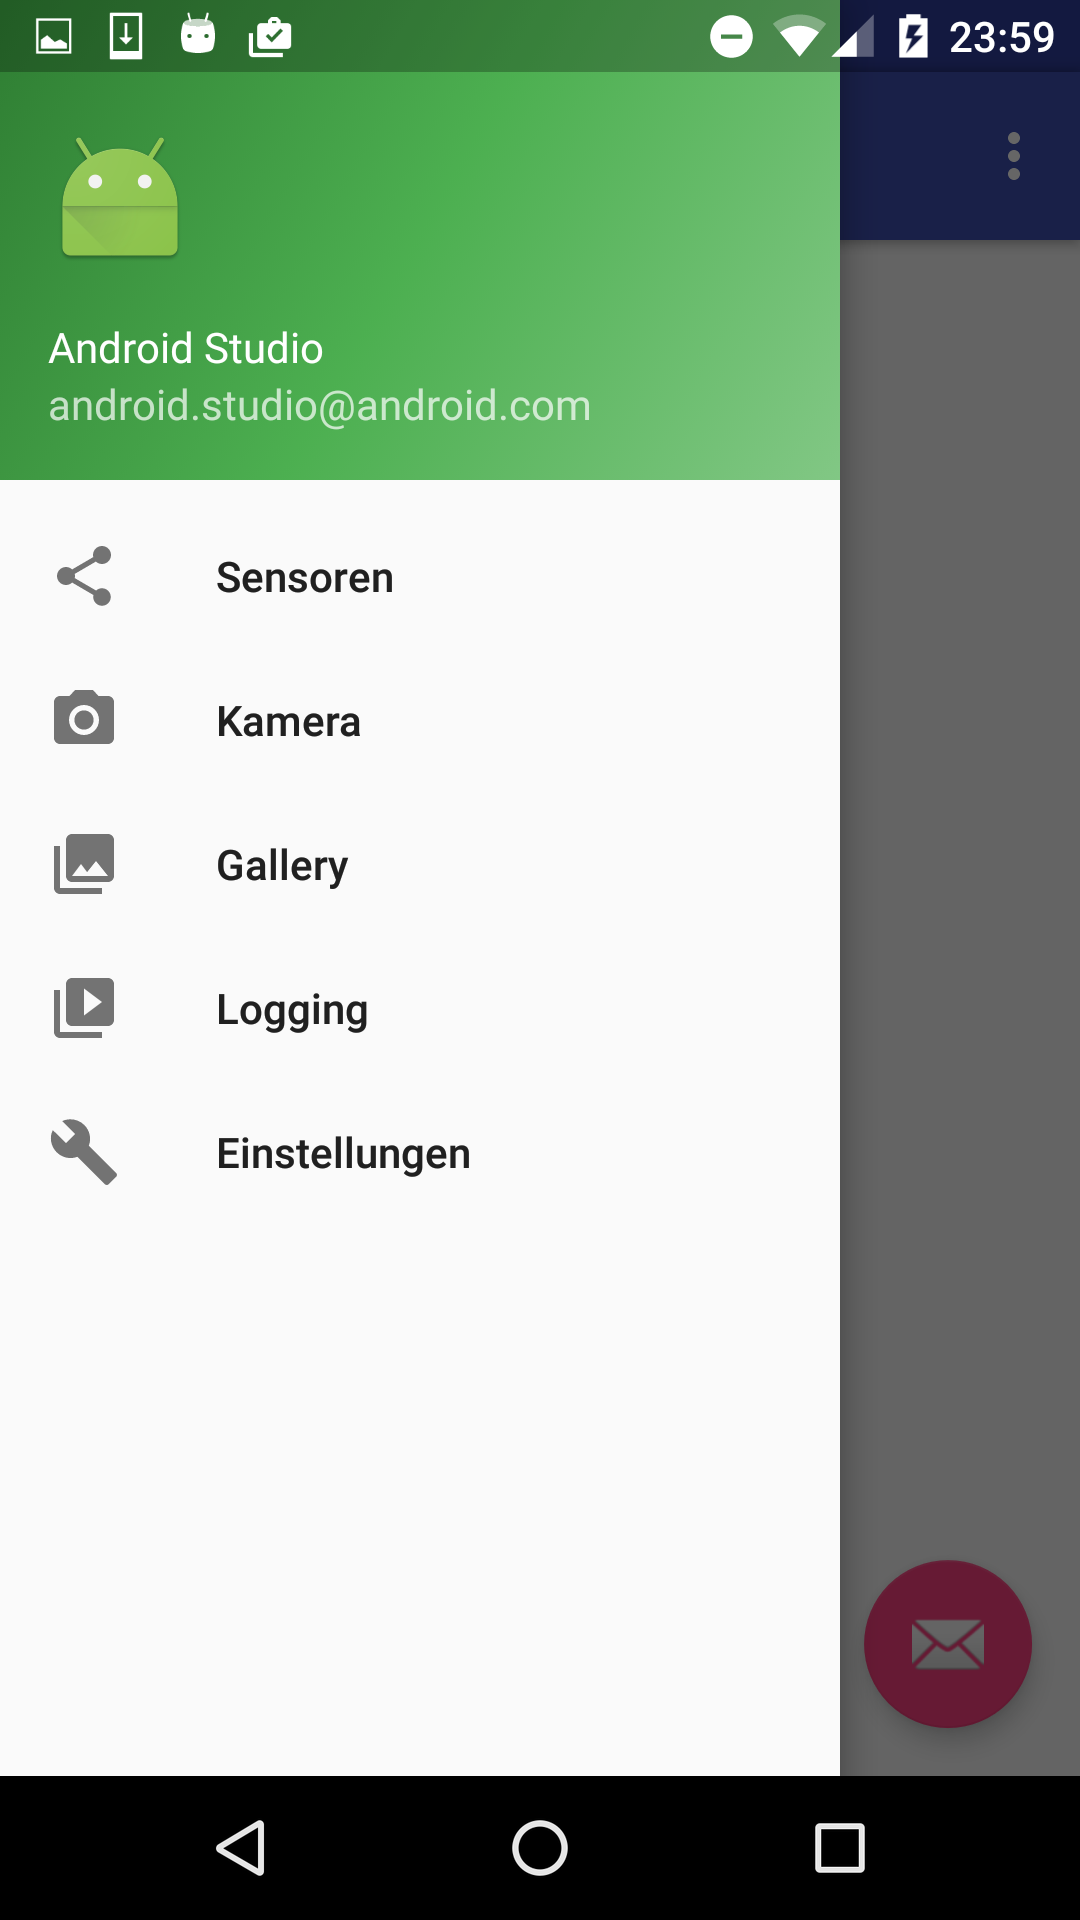
\includegraphics[width=0.4\textwidth]{Bilder/Screenshots/Screenshot_20170214-235908.PNG}
	\caption{Funktionstest-Anwendung: Startseite mit Hauptmenü}
	\label{fig:Main_Menu}
\end{figure}

Wählt der Benutzer im Hauptmenü die Kamerafunktion aus, so wechselt die Anwendung direkt in den Aufnahmemodus. In diesem Modus erscheint das Bild, welches die Kamera aufnimmt im Hintergrund. Vordergründig gibt es einen Auslöse-Button und einen Button für das Wechseln der Kameras im unteren Bildbereich. Ganz oben rechts sind die Blitzfunktionen, durch welche durch klicken navigiert werden kann. 
\\
\\
BILD
\\
\\
In der Galerie (siehe Abbildung \ref{fig:Gallery}) werden dem Benutzer die aufgenommenen und gespeicherten Bilder angezeigt. Durch diese Anzeige kann gescrollt werden. Einzelne Bilder können durch Klicken auf diese ausgewählt werden. Wird ein Bild angeklickt, so bekommt der Benutzer dieses in einem neuen Fenster groß angezeigt. Über den 'Floating Action Button' kann er nun dieses Bild löschen. 

\begin{figure}[h]
	\centering
	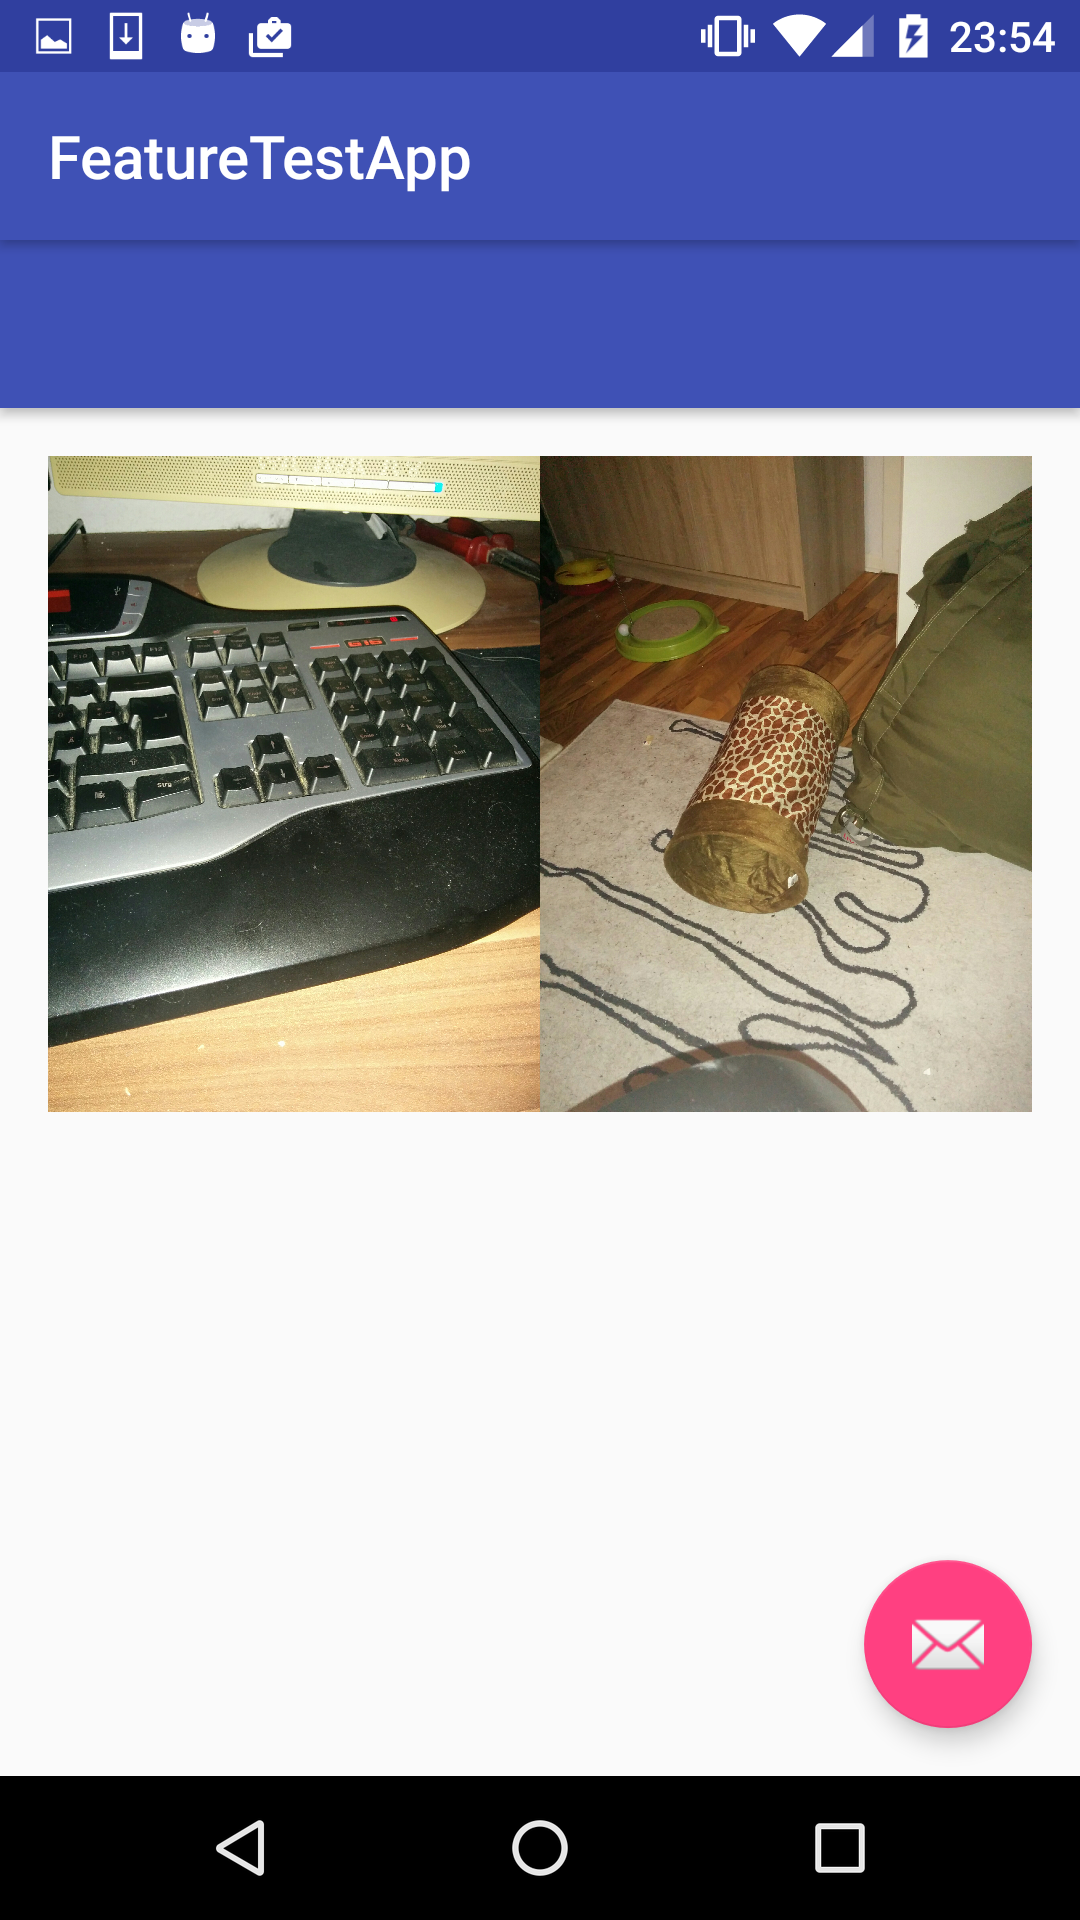
\includegraphics[width=0.4\textwidth]{Bilder/Screenshots/Screenshot_20170214-235454.PNG}
	\caption{Funktionstest-Anwendung: Galerie}
	\label{fig:Gallery}
\end{figure}

Wählt der Benutzer die Standortbestimmung aus, so erscheint im Hintergrund der Seite eine Weltkarte. Ist der Standort vom GPS-Sensor ermittelt worden, so erscheint ein MArker an diesem Ort auf der Weltkarte und die Kartenansicht schwenkt dorthin (siehe Abbildung \ref{fig:GPS}). Der Benutzer hat nun die Möglichkeit weiter in die Karte hinein zu zoomen, um den genauen Standort angezeigt zu bekommen. 
\clearpage

\begin{figure}[h]
	\centering
	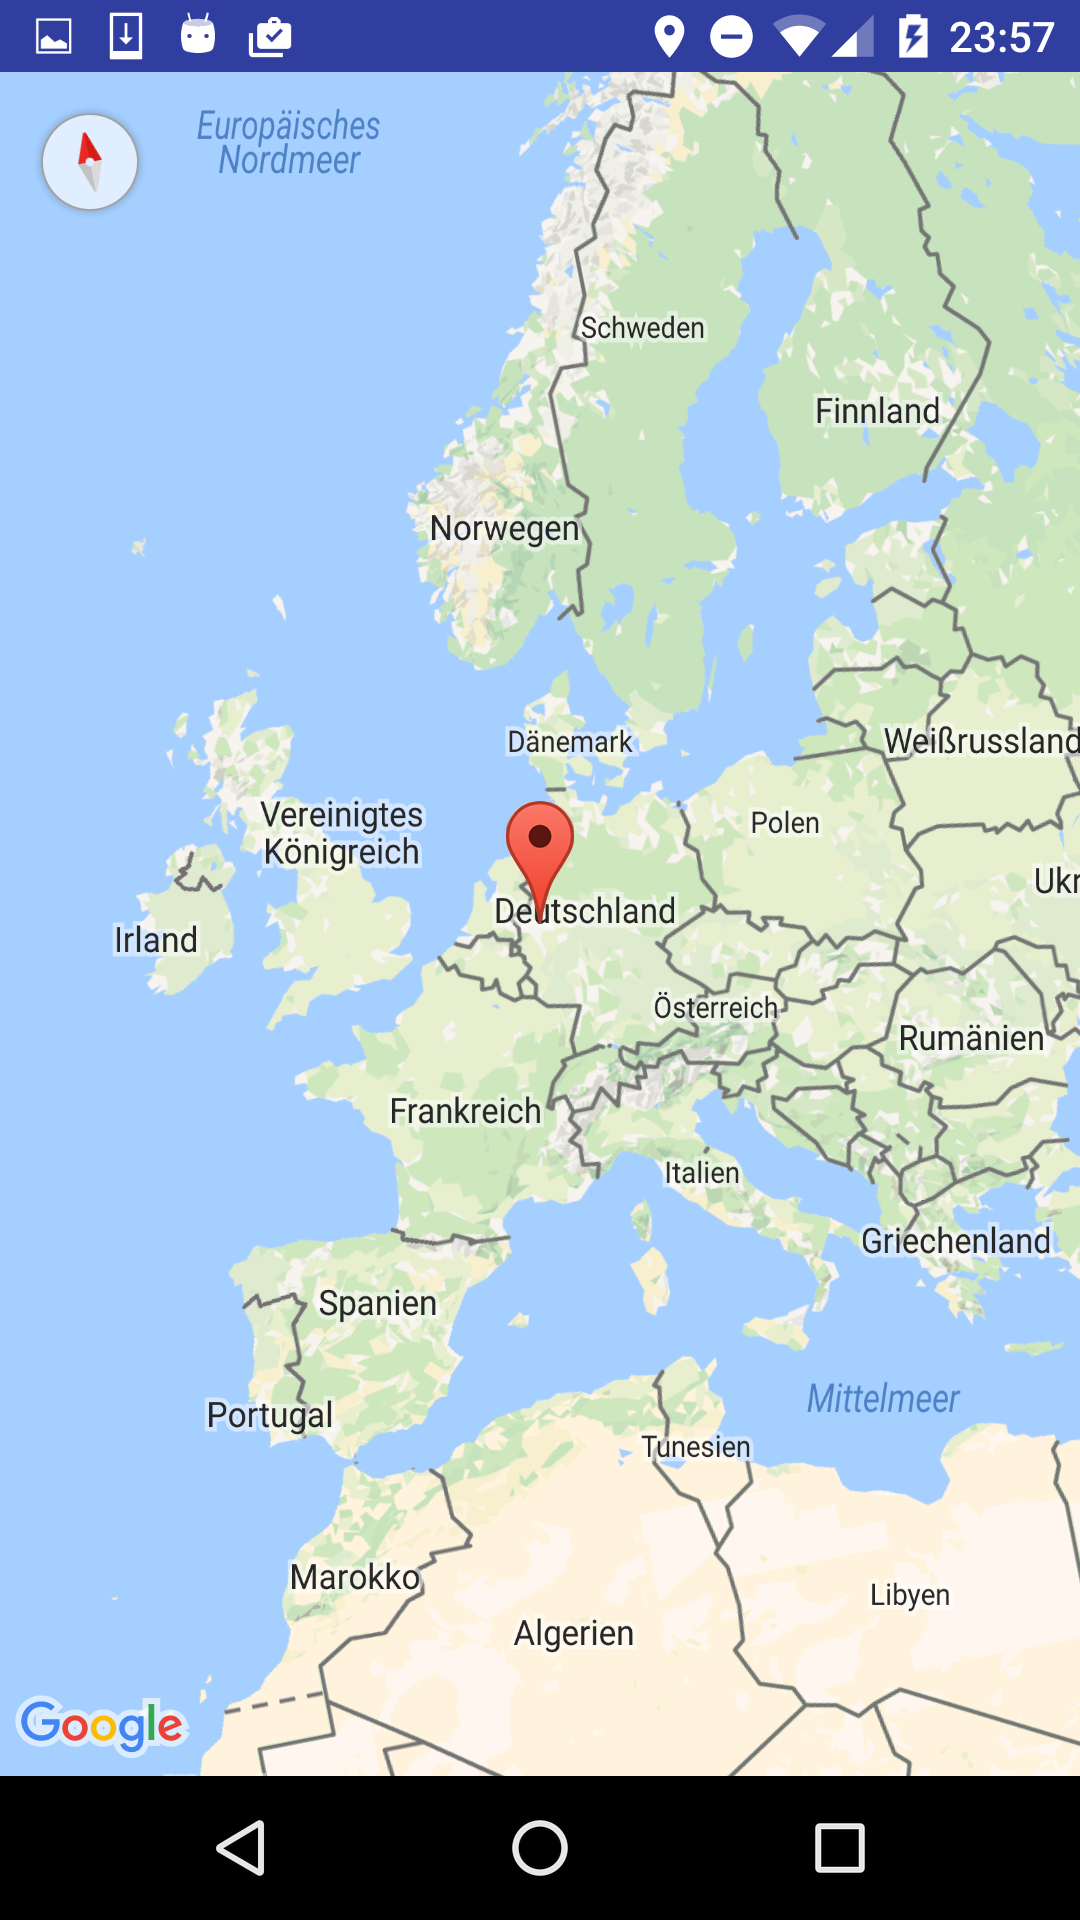
\includegraphics[width=0.4\textwidth]{Bilder/Screenshots/Screenshot_20170214-235726.PNG}
	\caption{Funktionstest-Anwendung: Standortbestimmung}
	\label{fig:GPS}
\end{figure}

Wird die Kompassfunktion gestartet, wird automatisch vom im Smartphone verbauten Magnetometer der magnetische Nordpol ermittelt. Auf der Anzeige wird dem Benutzer eine Kompassrose angezeigt, welche mit der 'N'-Spitze in Richtung magnetischen Nordpol zeigt (siehe Abbildung \ref{fig:Compass}).
\clearpage

\begin{figure}[h]
	\centering
	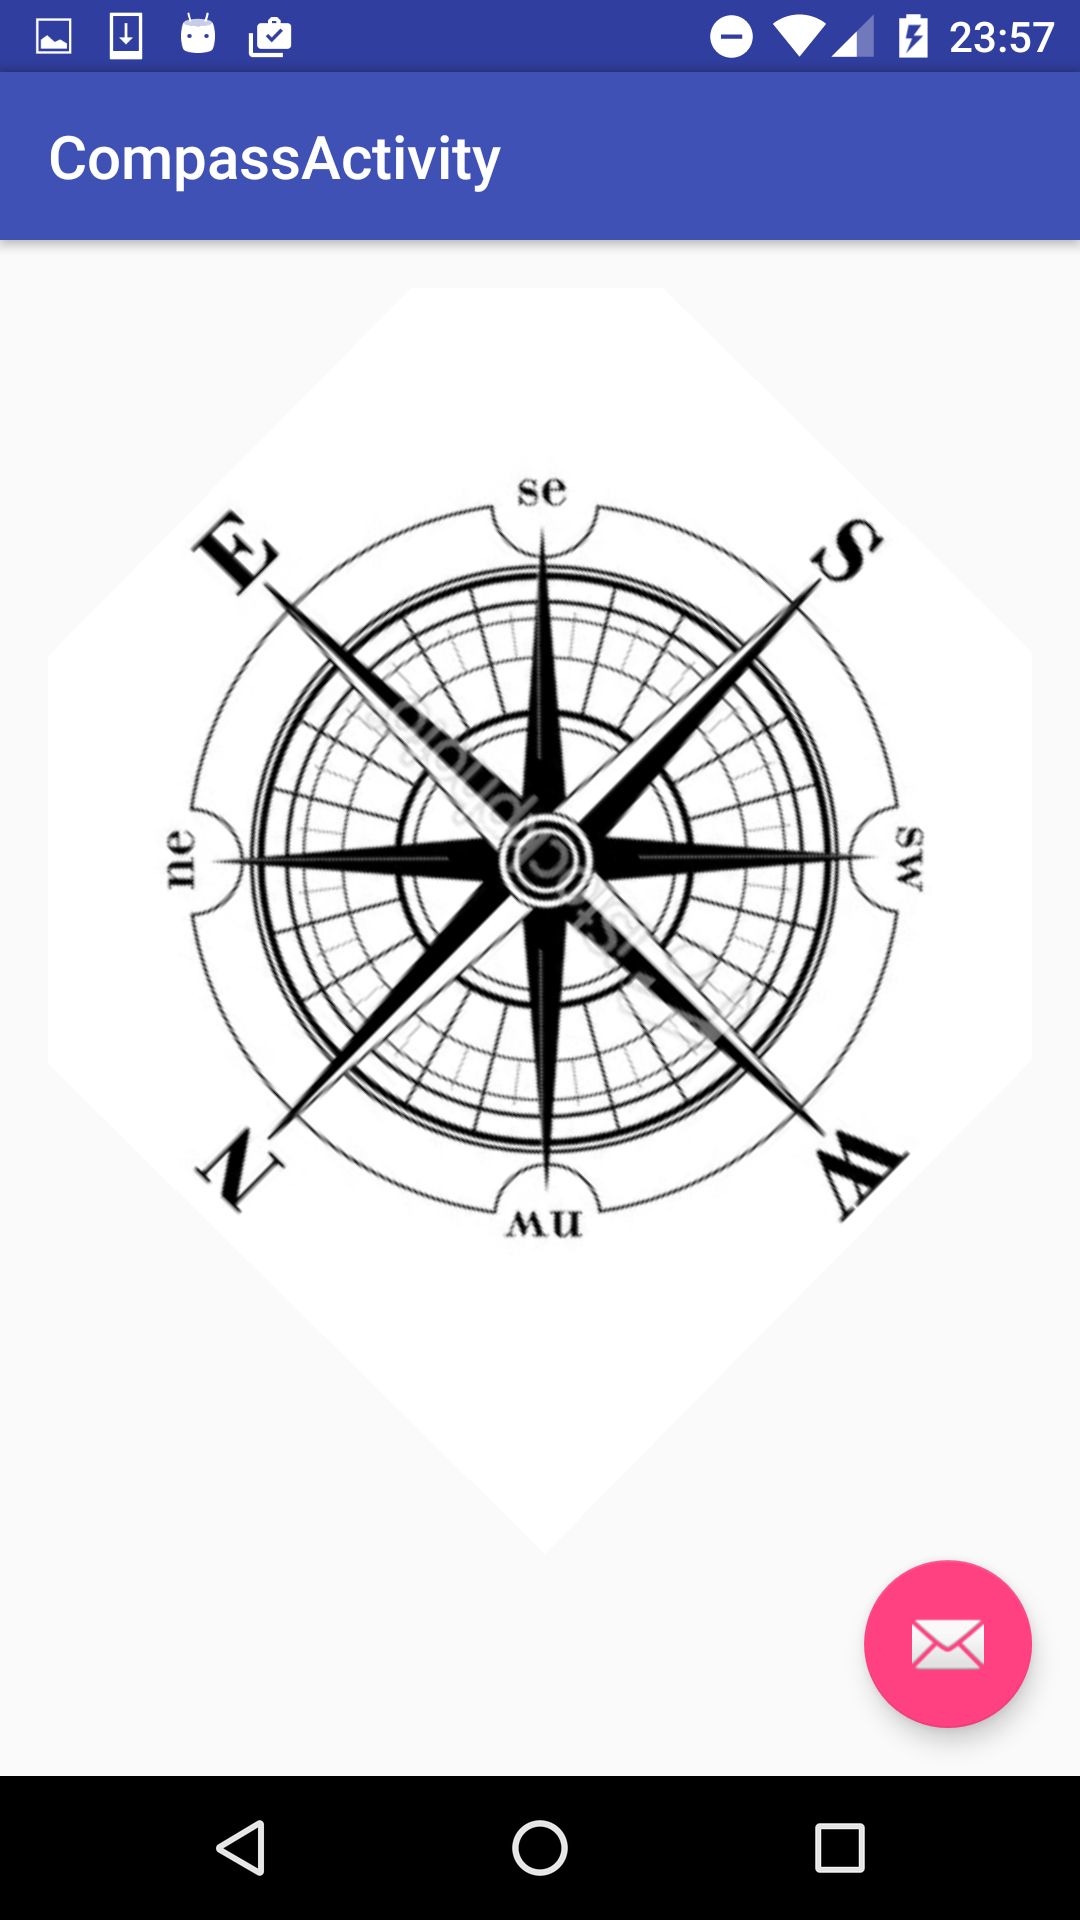
\includegraphics[width=0.4\textwidth]{Bilder/Screenshots/Screenshot_20170214-235753.PNG}
	\caption{Funktionstest-Anwendung: Kompassfunktion}
	\label{fig:Compass}
\end{figure}

Auf der Seite des Bewegungstests werden die vom Beschleunigungssensor ausgelesenen Daten angezeigt. Die Beschleunigungen werden dabei, wie in Kapitel (X) beschrieben, je Achse angegeben. Zusätzlich zur angezeigten momentanen Beschleunigung werden noch die Werte der maximalen Beschleunigung angezeigt und aktuell gehalten (siehe Abbildung \ref{fig:Accelerometer}). Ein separater Lagesensor wird an dieser Stelle nicht getestet, der Sensortyp 'ORIENTATION' ist veraltet. Anhand des Achsenmodells des Beschleunigungssensors kann die Lage des Smartphones erkannt werden. 
\clearpage

\begin{figure}[h]
	\centering
	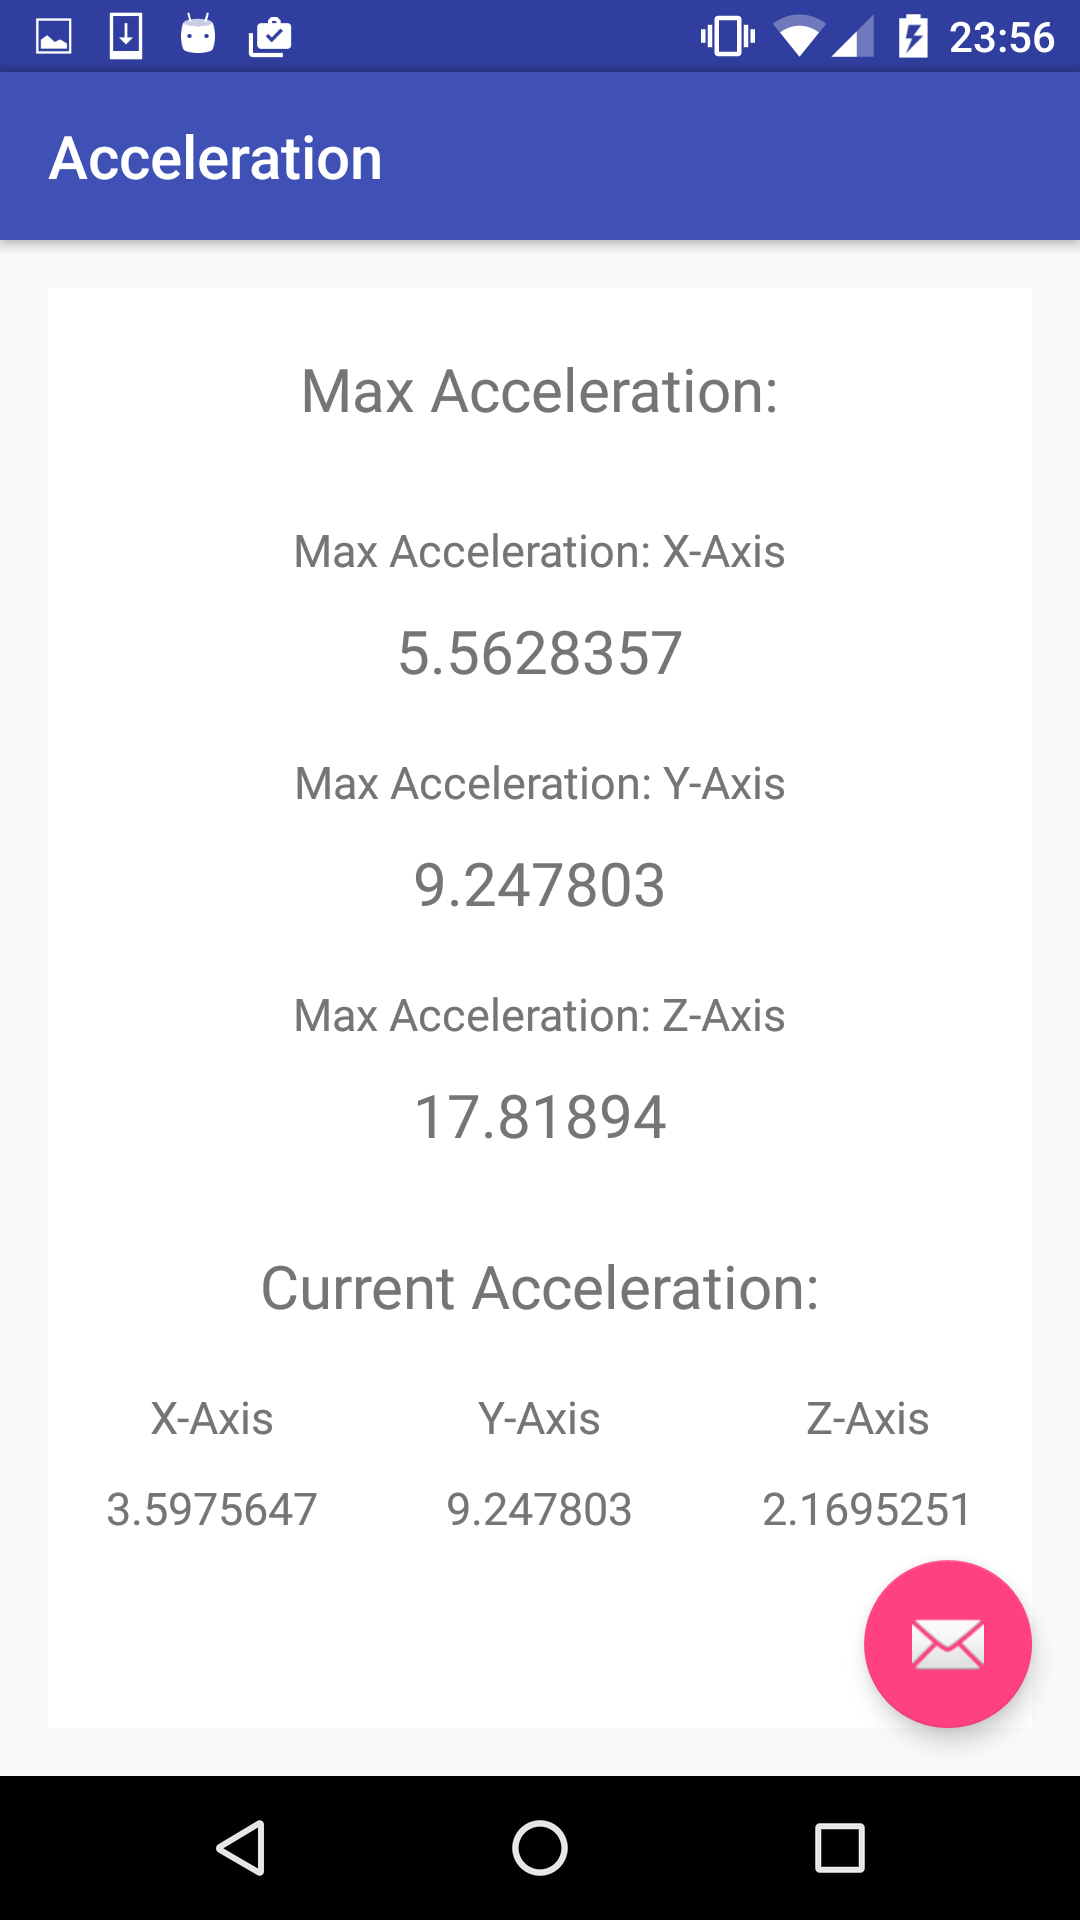
\includegraphics[width=0.4\textwidth]{Bilder/Screenshots/Screenshot_20170214-235635.PNG}
	\caption{Funktionstest-Anwendung: Bewegungstest}
	\label{fig:Accelerometer}
\end{figure}

Bei dem Test des Näherungssensors werden die ausgewerteten Sensordaten an ein 'Toast'-Objekt übergeben. Dieser 'Toast' zeigt 'far' an, wenn sich kein Objekt nahe vor dem Display des Smartphones befindet, und 'near' wenn sich eines genähert hat (siehe Abbildung \ref{fig:Proximity}).

 \clearpage

\begin{figure}[h]
	\centering
	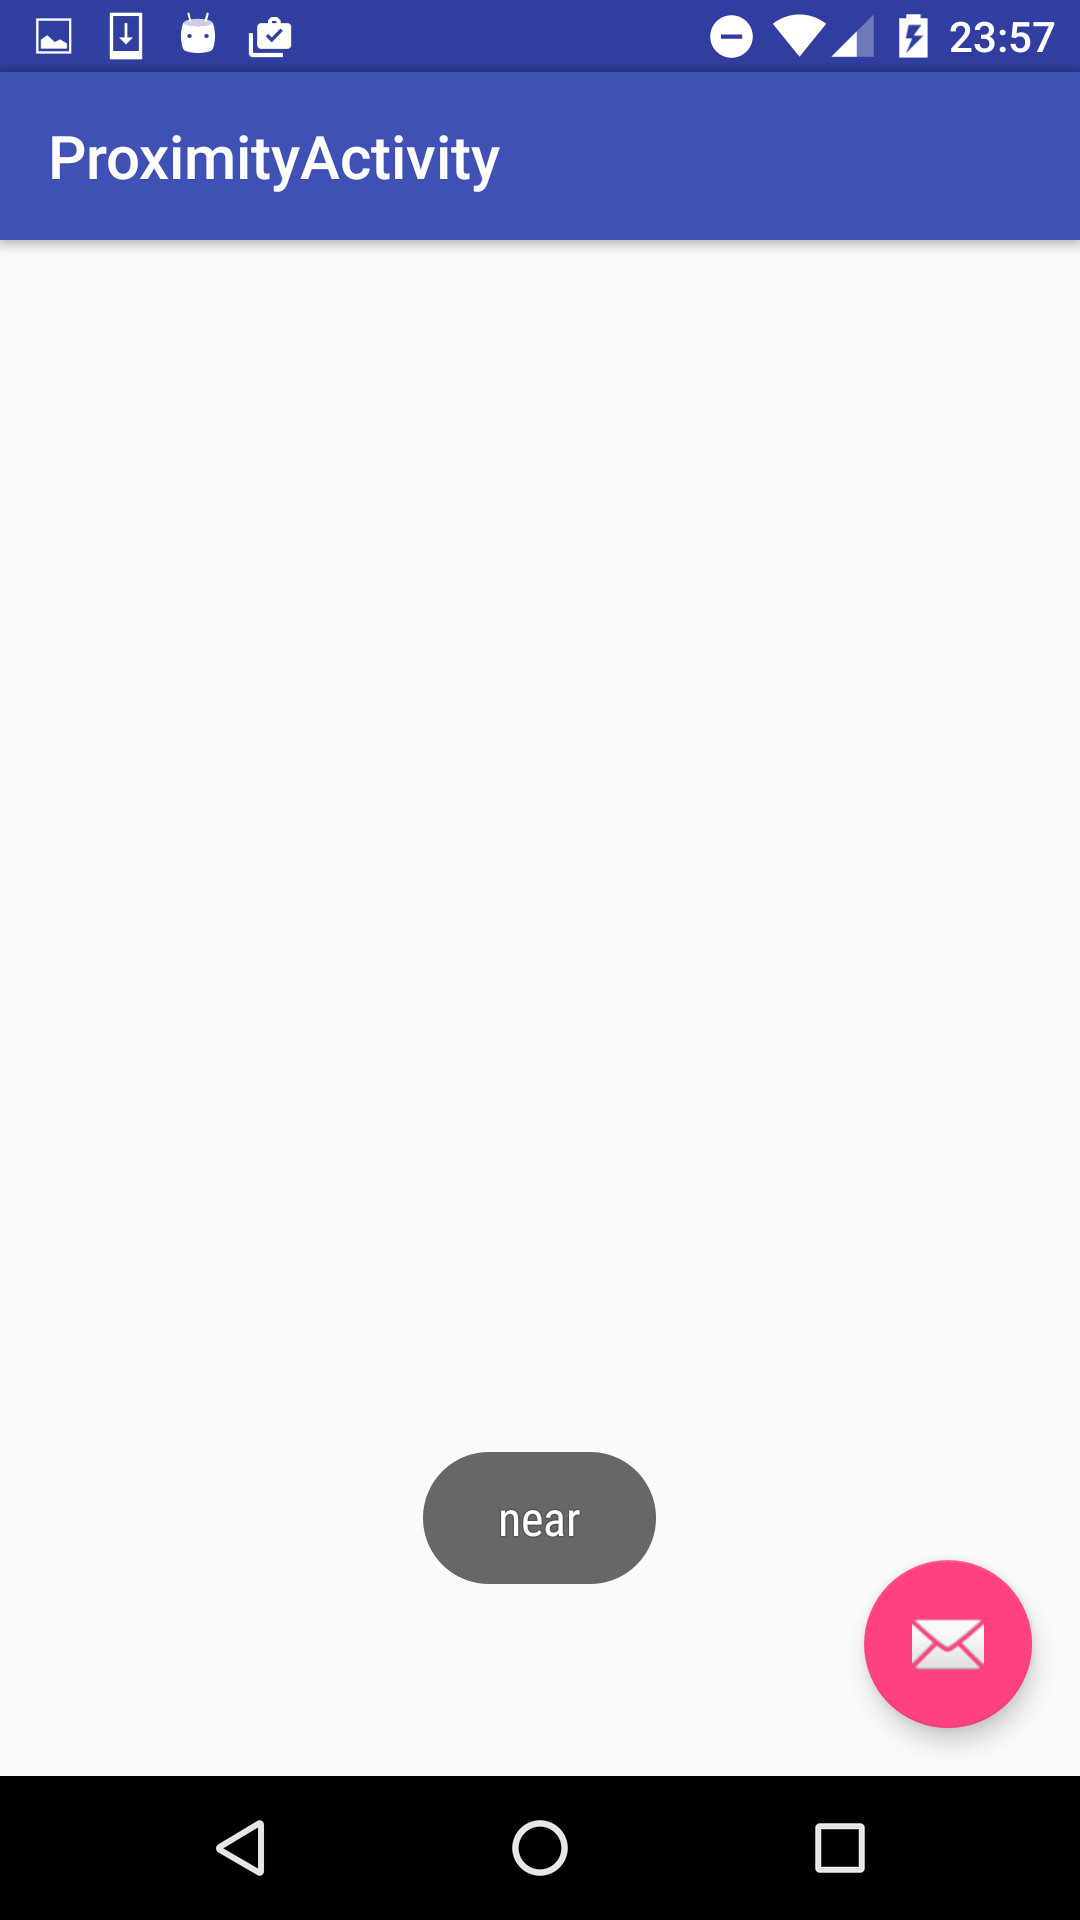
\includegraphics[width=0.4\textwidth]{Bilder/Screenshots/Screenshot_20170214-235744.PNG}
	\caption{Funktionstest-Anwendung: Näherungstest}
	\label{fig:Proximity}
\end{figure}